\documentclass{beamer}
\usepackage[T1]{fontenc}
\usepackage[utf8]{inputenc}
\usepackage{graphicx}
\usepackage[normalem]{ulem}
\usepackage{xmpmulti}
\usepackage{marvosym}
% \usepackage[dvipsnames]{xcolor}
% \usepackage{enumitem}

\DeclareMathOperator{\td}{td}
\DeclareMathOperator{\ld}{ld}
\DeclareMathOperator{\bw}{bw}
\DeclareMathOperator{\diam}{diam}
\DeclareMathOperator{\dist}{dist}
\newcommand{\emphh}[1]{\textcolor{blue}{\emph{#1}}}
\newcommand{\hilite}[1]{\emphh{#1}}
\title{Planar Graphs in Blowups of Fans \\
Using Product Structure with Metric Embeddings}

\newcommand{\verteq}{\rotatebox{90}{$\equiv$}}

\author{}
\author{\only<1>{%
  Marc Distel \and
  Vida~Dujmović \and
  Gwenaël~Joret \newline \and
  Piotr~Micek \and
  Pat Morin \and
  David R. Wood}%
  \only<2>{%
    Gwenaël~Joret \and
    Pat Morin \and
    David R. Wood \newline \and
    Vida~Dujmović \and
    Piotr~Micek \and
    Marc Distel}%
     \\[3ex]
  \only<1>{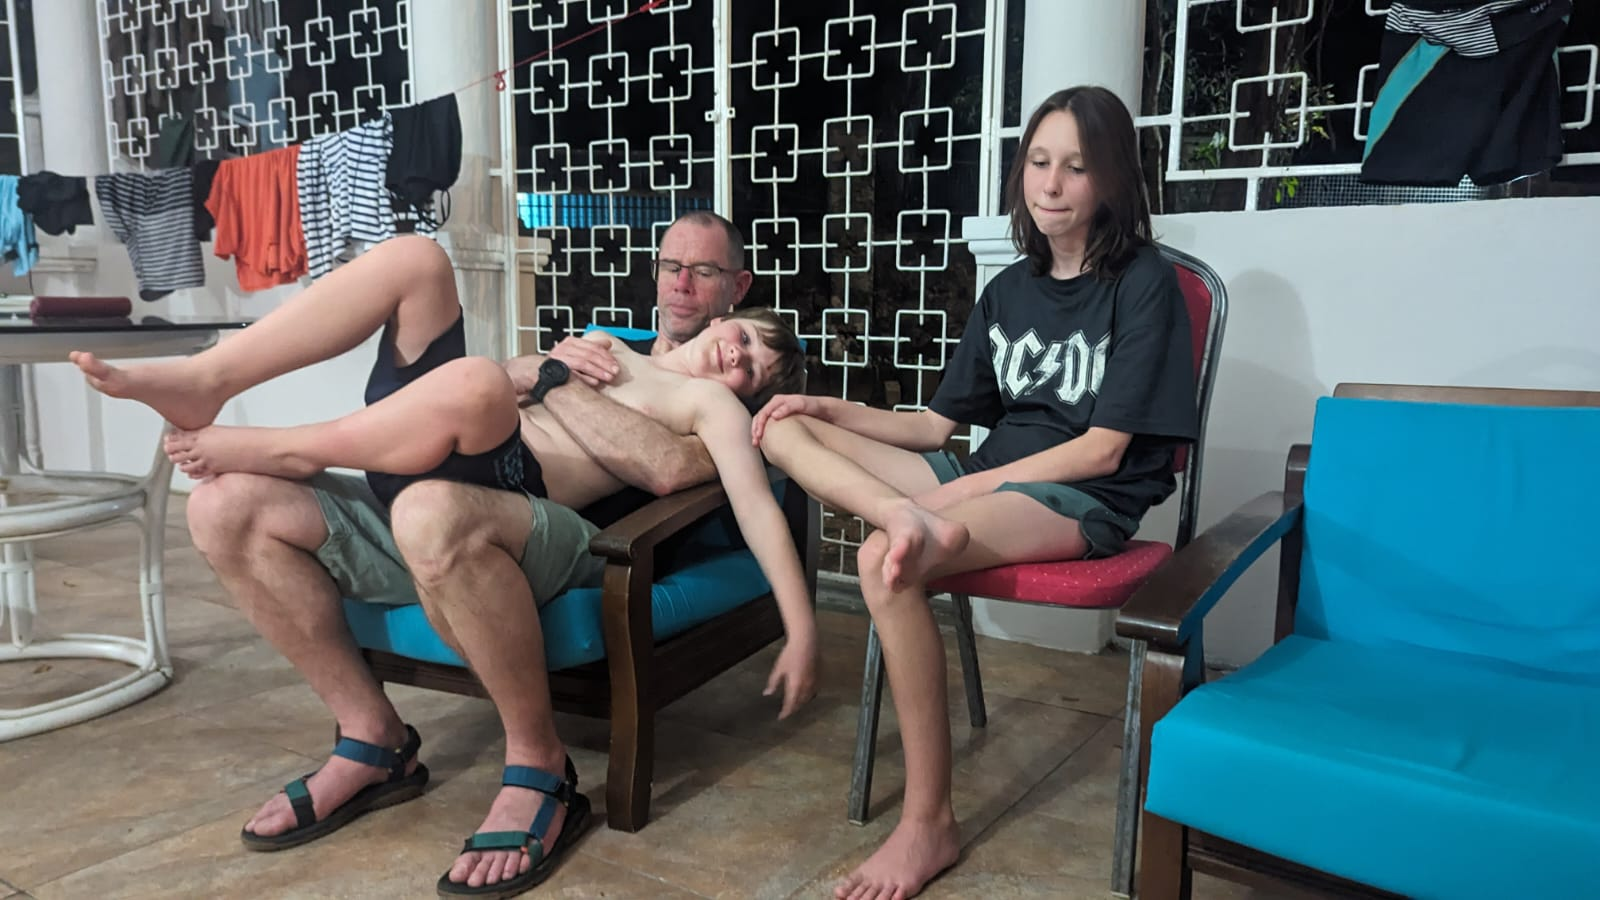
\includegraphics[height=.428\textheight]{images/pat-and-kids}\\(How we started)}
  %
  \only<2>{
\includegraphics[height=.428\textheight]{images/authors}
\includegraphics[height=.428\textheight]{images/marc-cropped}\\(How we finished)}%
}
\date{}

\setbeameroption{hide notes} % Only slides
%\setbeameroption{show only notes} % Only notes
% \setbeameroption{show notes on second screen=right} % Both


% \DeclareMathOperator{\tw}{tw}
% \DeclareMathOperator{\td}{td}
% \DeclareMathOperator{\wcol}{wcol}
% \DeclareMathOperator{\lvr}{\chi_{\ell-\mathrm{vr}}}
% \DeclareMathOperator{\pcn}{\chi_{p}}
\newcommand{\N}{\mathbb{N}}
\begin{document}

\begin{frame}
  % \begin{center}
    \maketitle
  % \end{center}
\end{frame}

\begin{frame}
  \frametitle{Contents}

  \begin{itemize}
    \item Planar graphs
    \item Product-structured graphs
    \item $K_t$-minor-free graphs
    \item Metric embeddings(!?)
    \item Summary, open problem
  \end{itemize}
\end{frame}

\begin{frame}
  \frametitle{Lipton-Tarjan Planar Separator Theorem}
  \framesubtitle{Lipton-Tarjan 1979}

  \begin{center}
    \only<1>{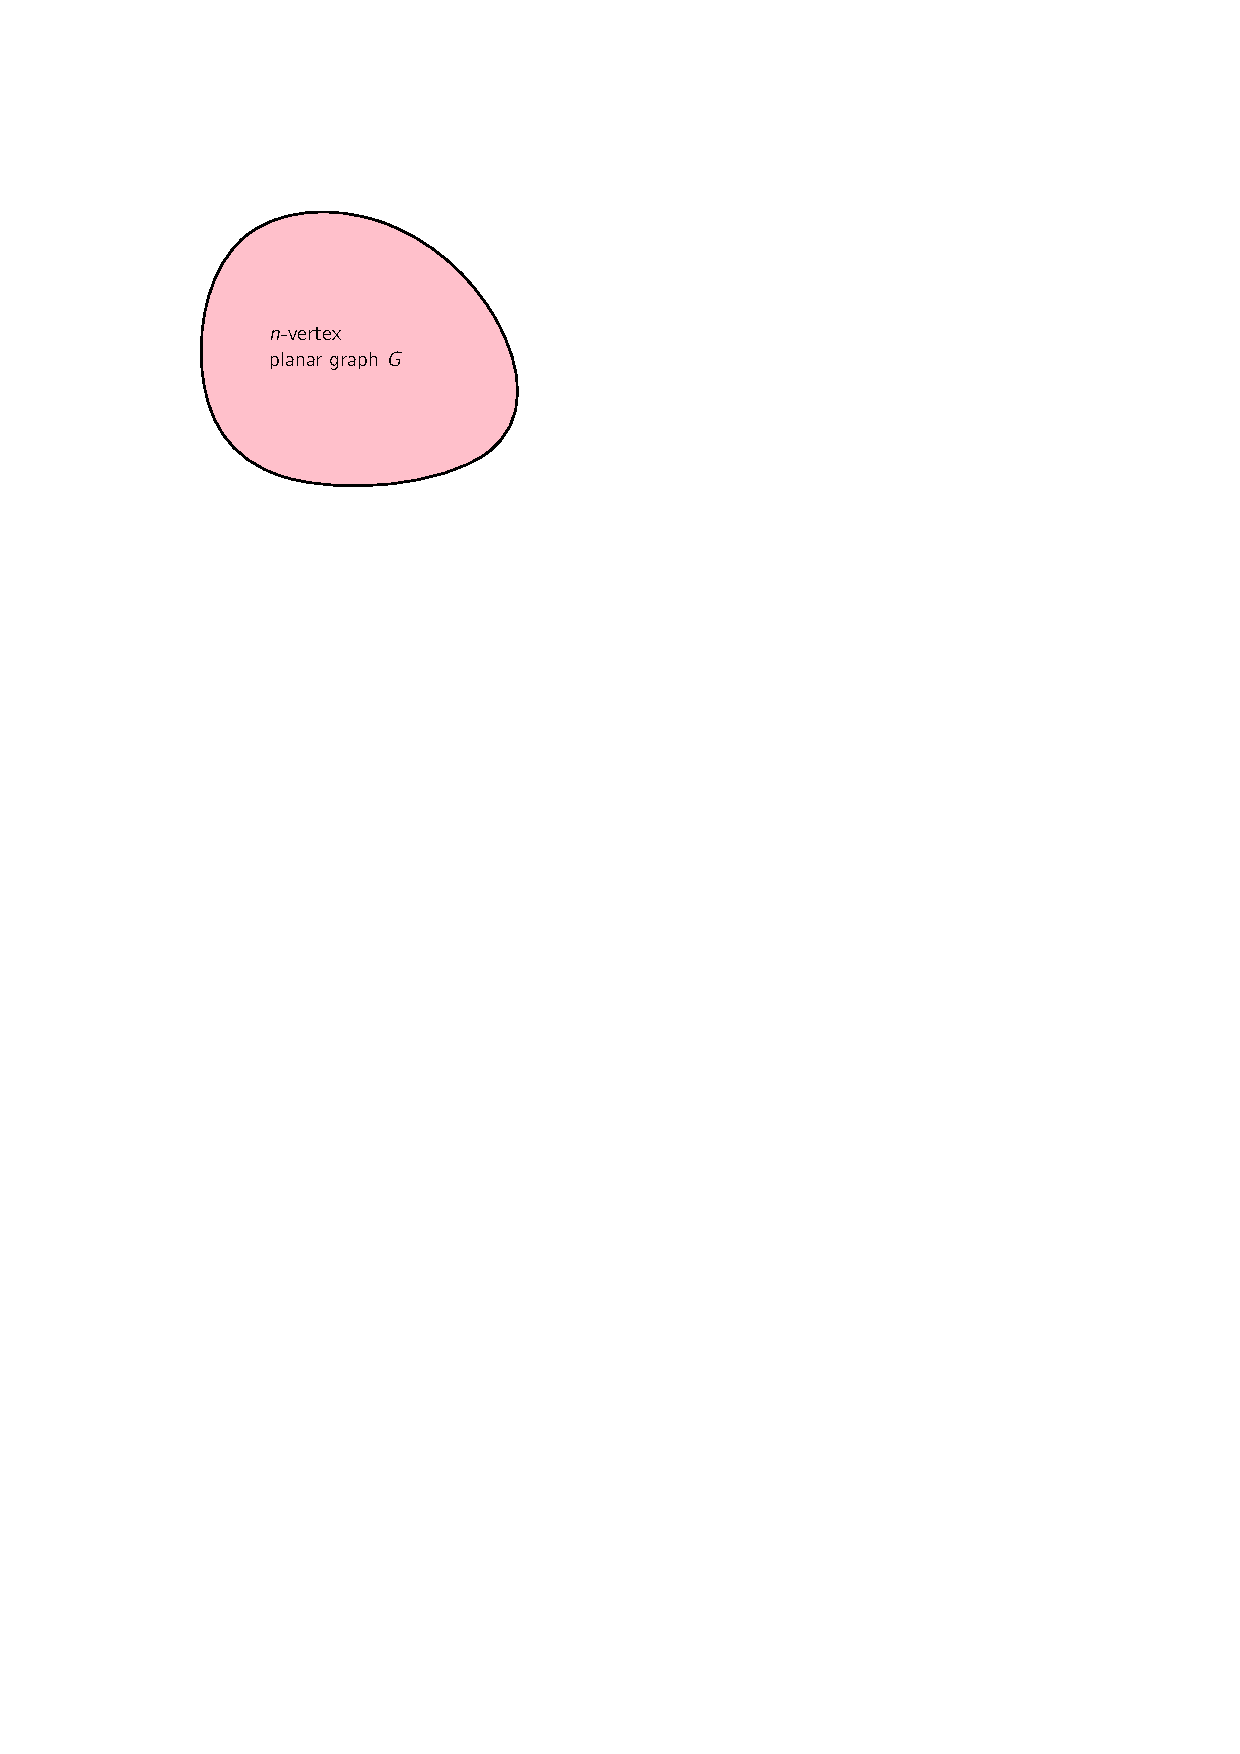
\includegraphics[page=1]{figs/lipton-tarjan-star}}%
    \only<2>{\includegraphics[page=2]{figs/lipton-tarjan-star}}%
    \only<3>{\includegraphics[page=3]{figs/lipton-tarjan-star}}%
    \only<4>{\includegraphics[page=4]{figs/lipton-tarjan-star}}%
    \only<5>{\includegraphics[page=5]{figs/lipton-tarjan-star}}%
    \only<6>{\includegraphics[page=6]{figs/lipton-tarjan-star}}%
    \only<7>{\includegraphics[page=7]{figs/lipton-tarjan-star}}%
    \only<8>{\includegraphics[page=8]{figs/lipton-tarjan-star}}%
    \only<9>{\includegraphics[page=9]{figs/lipton-tarjan-star}}%
    \only<10>{\includegraphics[page=10]{figs/lipton-tarjan-star}}%
    \only<11>{\includegraphics[page=11]{figs/lipton-tarjan-star}}%
    \only<12>{\includegraphics[page=12]{figs/lipton-tarjan-star}}%
    \only<13>{\includegraphics[page=13]{figs/lipton-tarjan-star}}%
    \only<14>{\includegraphics[page=14]{figs/lipton-tarjan-star}}%
    \only<15>{\includegraphics[page=15]{figs/lipton-tarjan-star}}%
    \only<16>{\includegraphics[page=16]{figs/lipton-tarjan-star}}%
    \only<17>{\includegraphics[page=17]{figs/lipton-tarjan-star}}%
    \only<18>{\includegraphics[page=18]{figs/lipton-tarjan-star}}%
    \only<19>{\includegraphics[page=19]{figs/lipton-tarjan-star}}%
    \only<20>{\includegraphics[page=20]{figs/lipton-tarjan-star}}%
    \only<21>{\includegraphics[page=21]{figs/lipton-tarjan-star}}%
    \only<22>{\includegraphics[page=22]{figs/lipton-tarjan-star}}%
    \only<23>{\includegraphics[page=23]{figs/lipton-tarjan-star}}%
    \only<24>{\includegraphics[page=24]{figs/lipton-tarjan-star}}%
    \only<25>{\includegraphics[page=25]{figs/lipton-tarjan-star}}%
  \end{center}
\end{frame}

\begin{frame}
  \frametitle{Two variations}
  \framesubtitle{Dvořák-Wood 2022}

  \begin{center}
    \includegraphics[page=10,trim={0 2.2cm 0 0},clip]{figs/lipton-tarjan-star}
  \end{center}
  \textbf{Theorem:}
  $G\subseteq H\boxtimes K_{O(\sqrt{n})}$ where $\td(H)=O(\log\log n)$
  \\[2ex]
  \textbf{Theorem:}
  $G\subseteq H\boxtimes K_{O(n^{1/2+\epsilon})}$ where $\td(H)=O(1/\epsilon)$
\end{frame}

\begin{frame}
  \frametitle{Treewidth-$2$ partitions}
  \framesubtitle{Distel-Dujmović-Eppstein-Hickingbotham-Joret-Micek-M-Seweryn-Wood 2022}

  \textbf{Question:} What is the simplest graph class $\mathcal{H}$ such that every $n$-vertex planar graph $G$ is a subgraph of $H\boxtimes K_{O(\sqrt{n})}$ for some $H\in\mathcal{H}$?\\[3ex]

  % \uncover<2->{\textbf{Theorem (Dvořák-Wood 2022):} $G\subseteq H\boxtimes K_{O(\sqrt{n})}$ for some graph $H$ of \textcolor{red}{treedepth $O(\log\log n)$}.
  % \\[3ex]
  \uncover<2->{\textbf{Theorem (DDEHJMMSW2022):} $G\subseteq H\boxtimes K_{O(\sqrt{n})}$ for some graph $H$ of \textcolor{red}{treewidth 2}.\\[3ex]}

  \uncover<3->{What is simpler than treewidth 2?}\\[3ex]

  \uncover<4->{Pathwidth 2?}
\end{frame}

\begin{frame}
  \frametitle{Main result}
  % \framesubtitle{Distel-Dujmović-Eppstein-Hickingbotham-Joret-Micek-M-Seweryn-Wood 2022}

  \only<1>{\textbf{Theorem 1:} Every $n$-vertex planar $G$ is a subgraph of $F\boxtimes K_{O(\sqrt{n}\log^2 n)}$, where $F$ is a \textcolor{red}{fan}.}%
  \only<2->{\textbf{Theorem 1:} Every $n$-vertex planar $G$ is a subgraph of $F\boxtimes K_{\tilde{O}(\sqrt{n})}$, where $F$ is a \textcolor{red}{fan}.}\\[2ex]

  \uncover<3->{\textbf{Theorem 1:} Every $n$-vertex planar $G$ has a \textcolor{red}{fan partition} of width $\tilde{O}(\sqrt{n})$.}\\[2ex]

  \uncover<4->{\textbf{Theorem 1:} Every $n$-vertex planar $G$ has a set $X$ of $\tilde{O}(\sqrt{n})$ vertices such that $G-X$ has a \textcolor{red}{path partition} of width $\tilde{O}(\sqrt{n})$}

  \begin{center}
    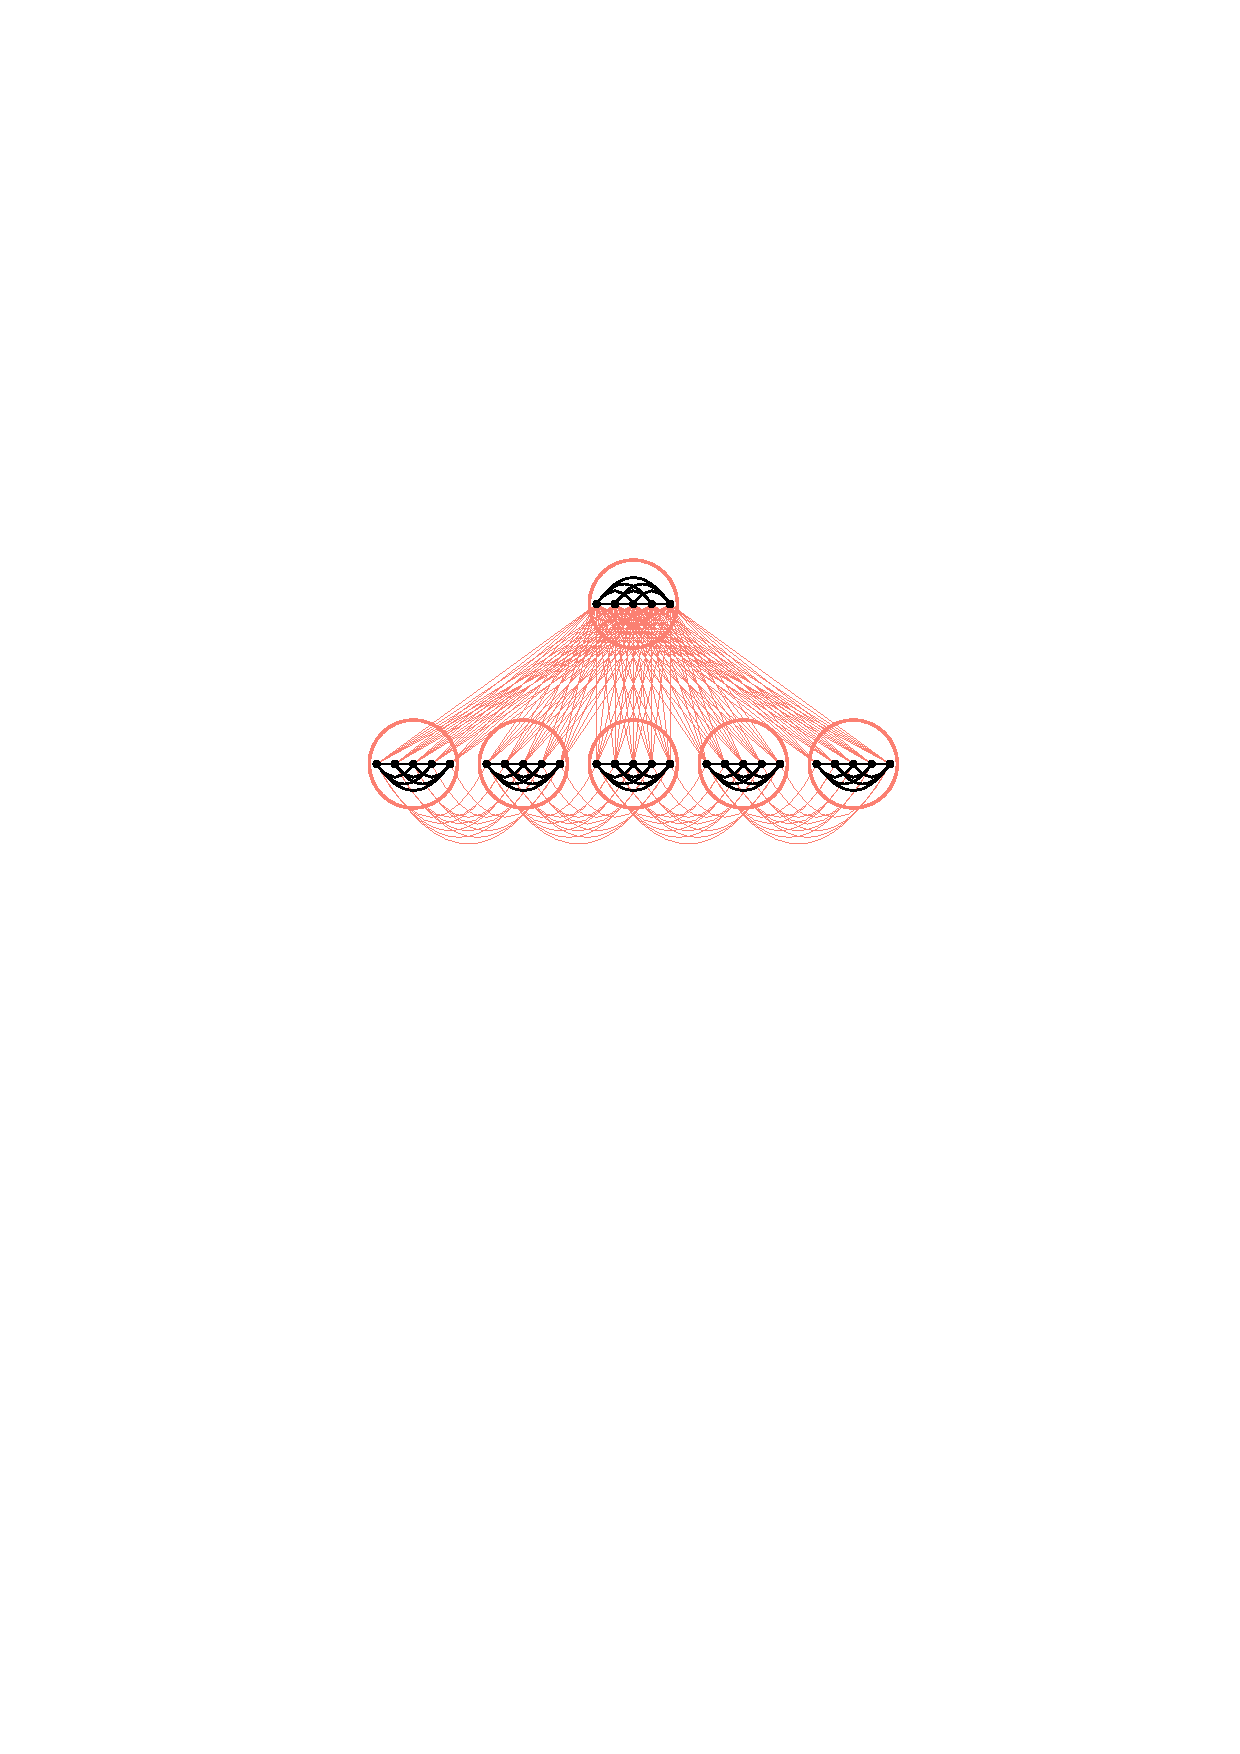
\includegraphics[width=.8\textwidth]{figs/fan-blowup}
  \end{center}
\end{frame}

\begin{frame}
  \frametitle{Path partitions and bandwidth}

  \uncover<1->{\textbf{Theorem 1:} Every $n$-vertex planar $G$ has a set $X$ of $\tilde{O}(\sqrt{n})$ vertices such that $G-X$ has a \textcolor{red}{path partition} of width $\tilde{O}(\sqrt{n})$}\\[2ex]

  \uncover<2->{\textbf{Theorem 1:} Every $n$-vertex planar $G$ has a set $X$ of $\tilde{O}(\sqrt{n})$ vertices such that $G-X$ has a \textcolor{red}{bandwidth} $\tilde{O}(\sqrt{n})$}

  \begin{center}
    \includegraphics[width=.8\textwidth,page=2]{figs/fan-blowup-slides}
  \end{center}

\end{frame}

\begin{frame}
  \frametitle{Obstacles to small bandwidth}

  \begin{tabular}{lr}
    \only<1>{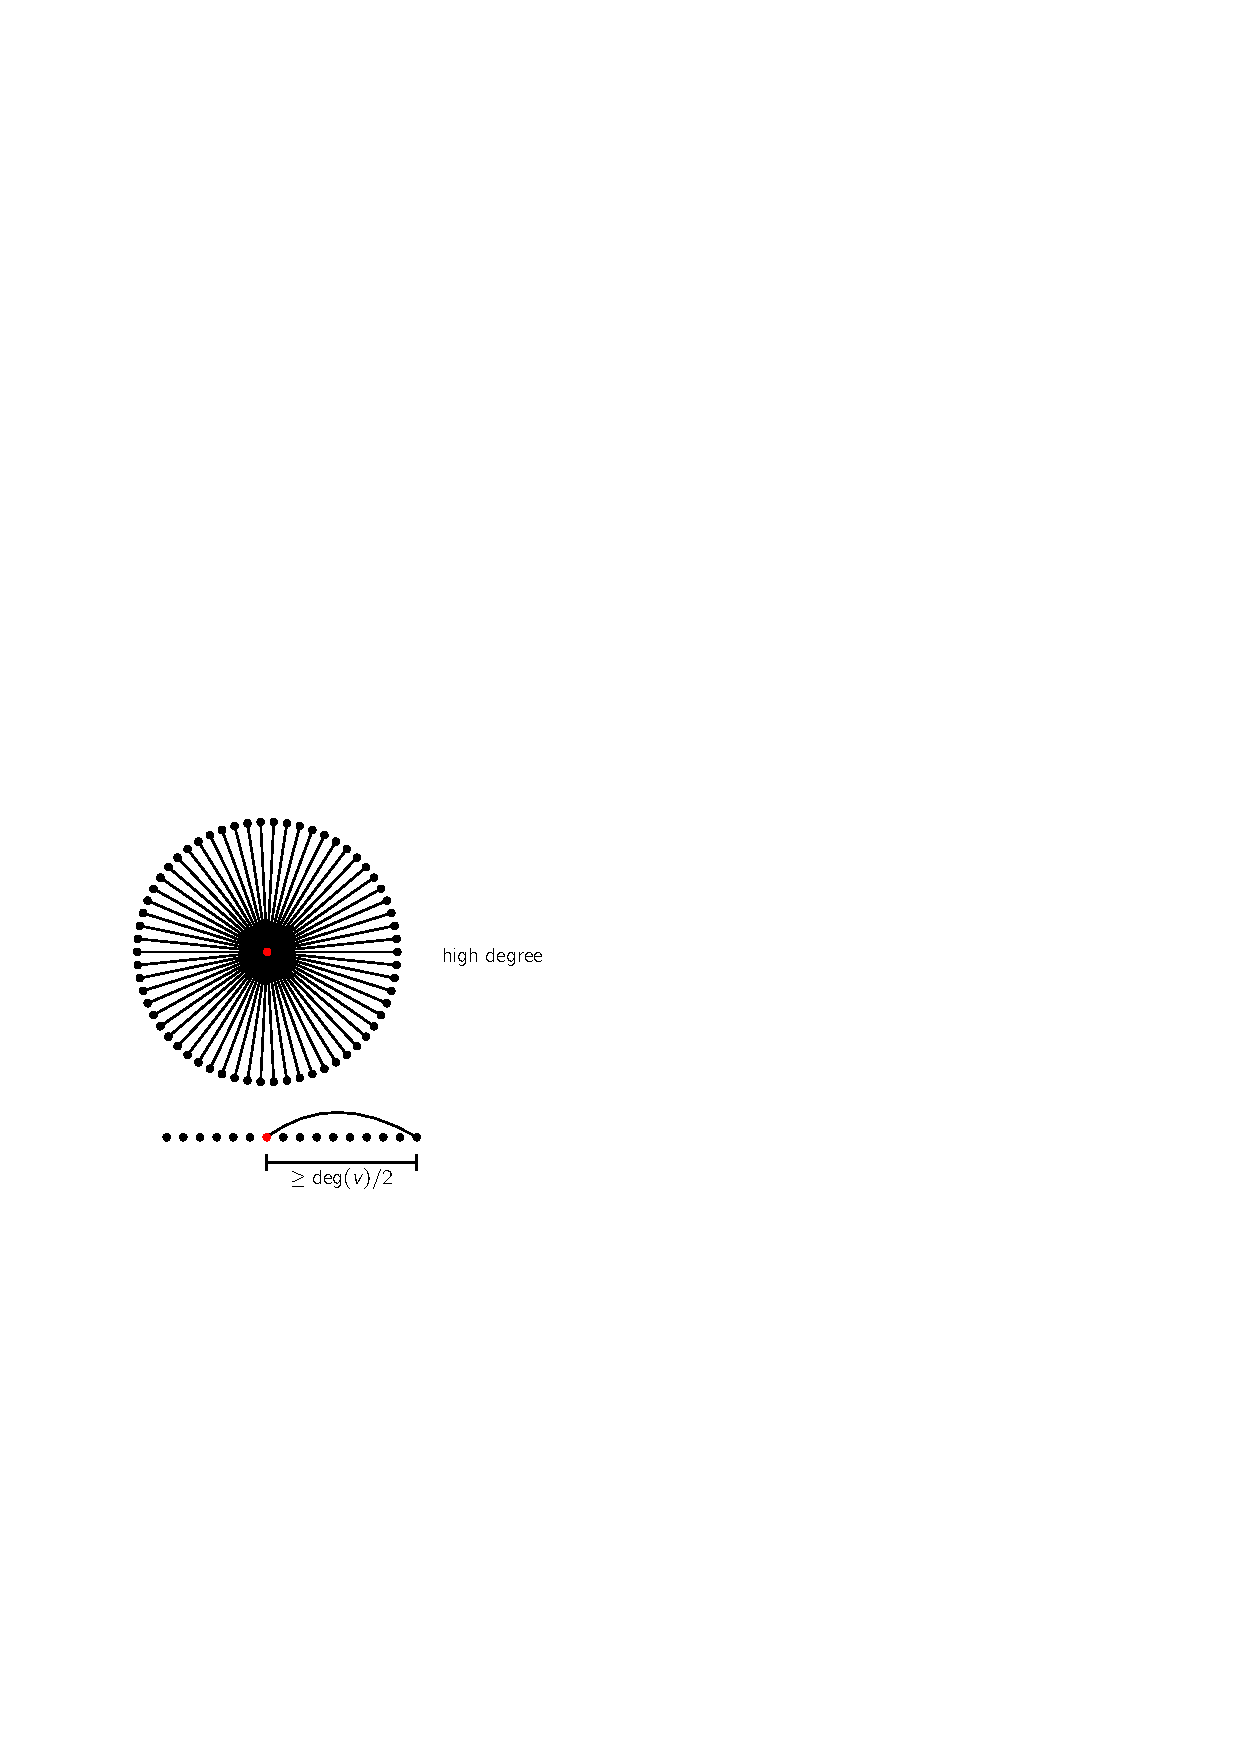
\includegraphics[page=1]{figs/bandwidth-obstacles}}%
    \only<2>{\includegraphics[page=2]{figs/bandwidth-obstacles}}%
    \only<3>{\includegraphics[page=3]{figs/bandwidth-obstacles}}%
    \only<4>{\includegraphics[page=4]{figs/bandwidth-obstacles}}% &
    \raisebox{5cm}{\includegraphics[width=.2\textwidth,page=2]{figs/fan-blowup-slides}}
  \end{tabular}
\end{frame}

\begin{frame}
  \frametitle{Local sparsification}

  \textbf{Theorem (Feige 2000):} If $G-X$ has local density $\tilde{O}(\sqrt{n})$ then $G-X$ has bandwidth $\tilde{O}(\sqrt{n})$.\\[3ex]

  \uncover<2->{\textbf{Goal:} Find $X\subseteq V(G)$ of size $\tilde{O}(\sqrt{n})$ so that every $r$-ball in $G-X$ contains $\tilde{O}(r\sqrt{n})$ vertices.}
\end{frame}

\begin{frame}
  \frametitle{Local sparsification}

  \only<1>{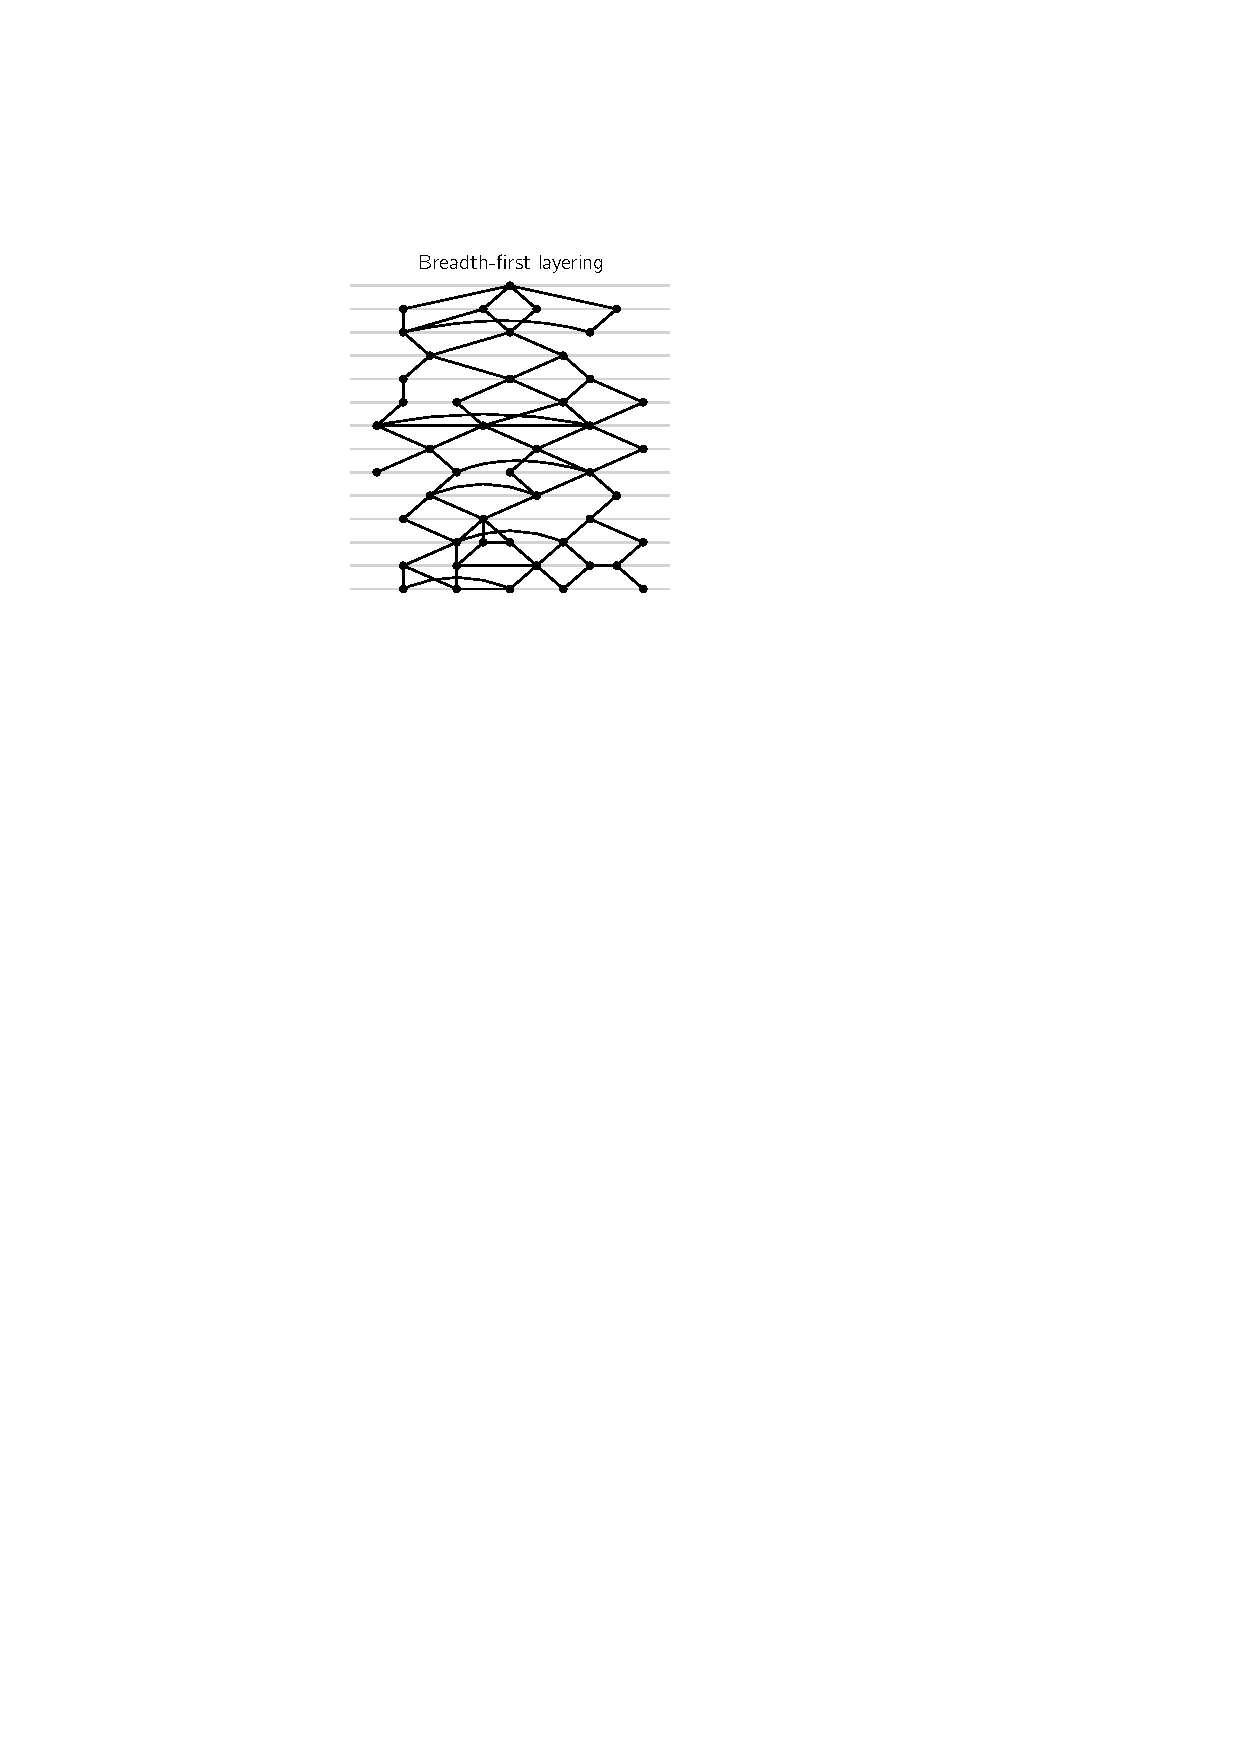
\includegraphics[page=1]{figs/layering}}%
  \only<2>{\includegraphics[page=2]{figs/layering}}%
  \only<3>{\includegraphics[page=3]{figs/layering}}%
  \only<4>{\includegraphics[page=4]{figs/layering}}%
  \only<5>{\includegraphics[page=5]{figs/layering}}%
  \only<6>{\includegraphics[page=6]{figs/layering}}%
  \only<7>{\includegraphics[page=7]{figs/layering}}%
  \only<8>{\includegraphics[page=8]{figs/layering}}%
  \only<9>{\includegraphics[page=9]{figs/layering}}%
  \only<10>{\includegraphics[page=10]{figs/layering}}%
\end{frame}

\begin{frame}
  \frametitle{Looking under the tilde}

  \begin{itemize}[<+->]
    \item Tradeoff:  $\ld(G-X)\le D \Leftrightarrow |X|\in O((n\log n)/D)$

    \item Feige: For \emphh{any} $G$, $\ld(G)\le D$ implies $\bw(G)\in O(D\log^3 n\sqrt{\log n\log\log n})$

    \item Rao (Better): For \emphh{planar} $G$, $\ld(G)\le D$ implies $\bw(G)\in O(D\log^3 n)$

    \item Take $D=\sqrt{n}/\log n$, so $|X|\in O(\sqrt{n}\log^2 n)$ and $\bw(G-X)\in O(\sqrt{n}\log^2 n)$.

    \item For any planar $G$, $G\subseteq F\boxtimes K_{O(n\log^2 n)}$
  \end{itemize}
\end{frame}


\begin{frame}
  \frametitle{Product Structure}
  % \framesubtitle{Planar graphs and beyond}

  \begin{center}
  \only<1>{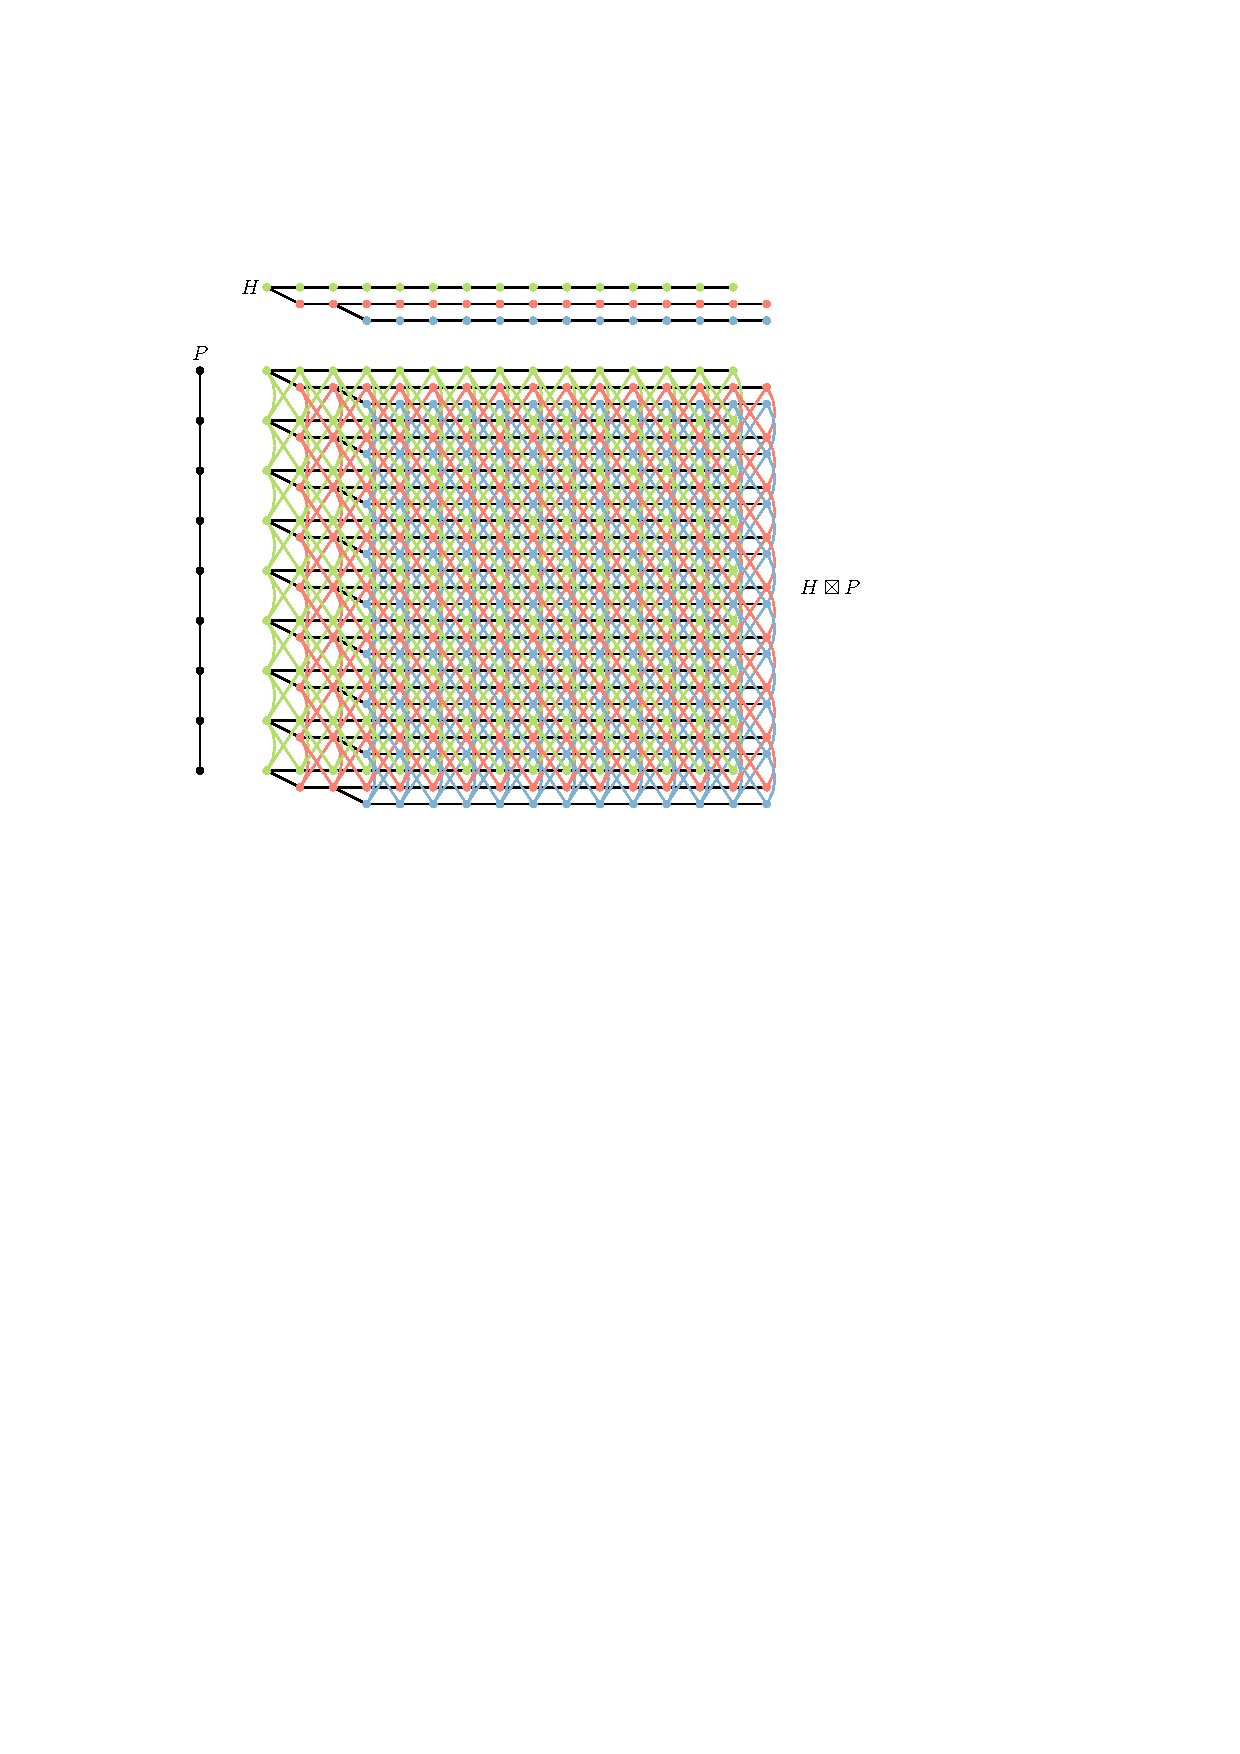
\includegraphics[height=.6\textheight]{figs/product}}%
  \only<2->{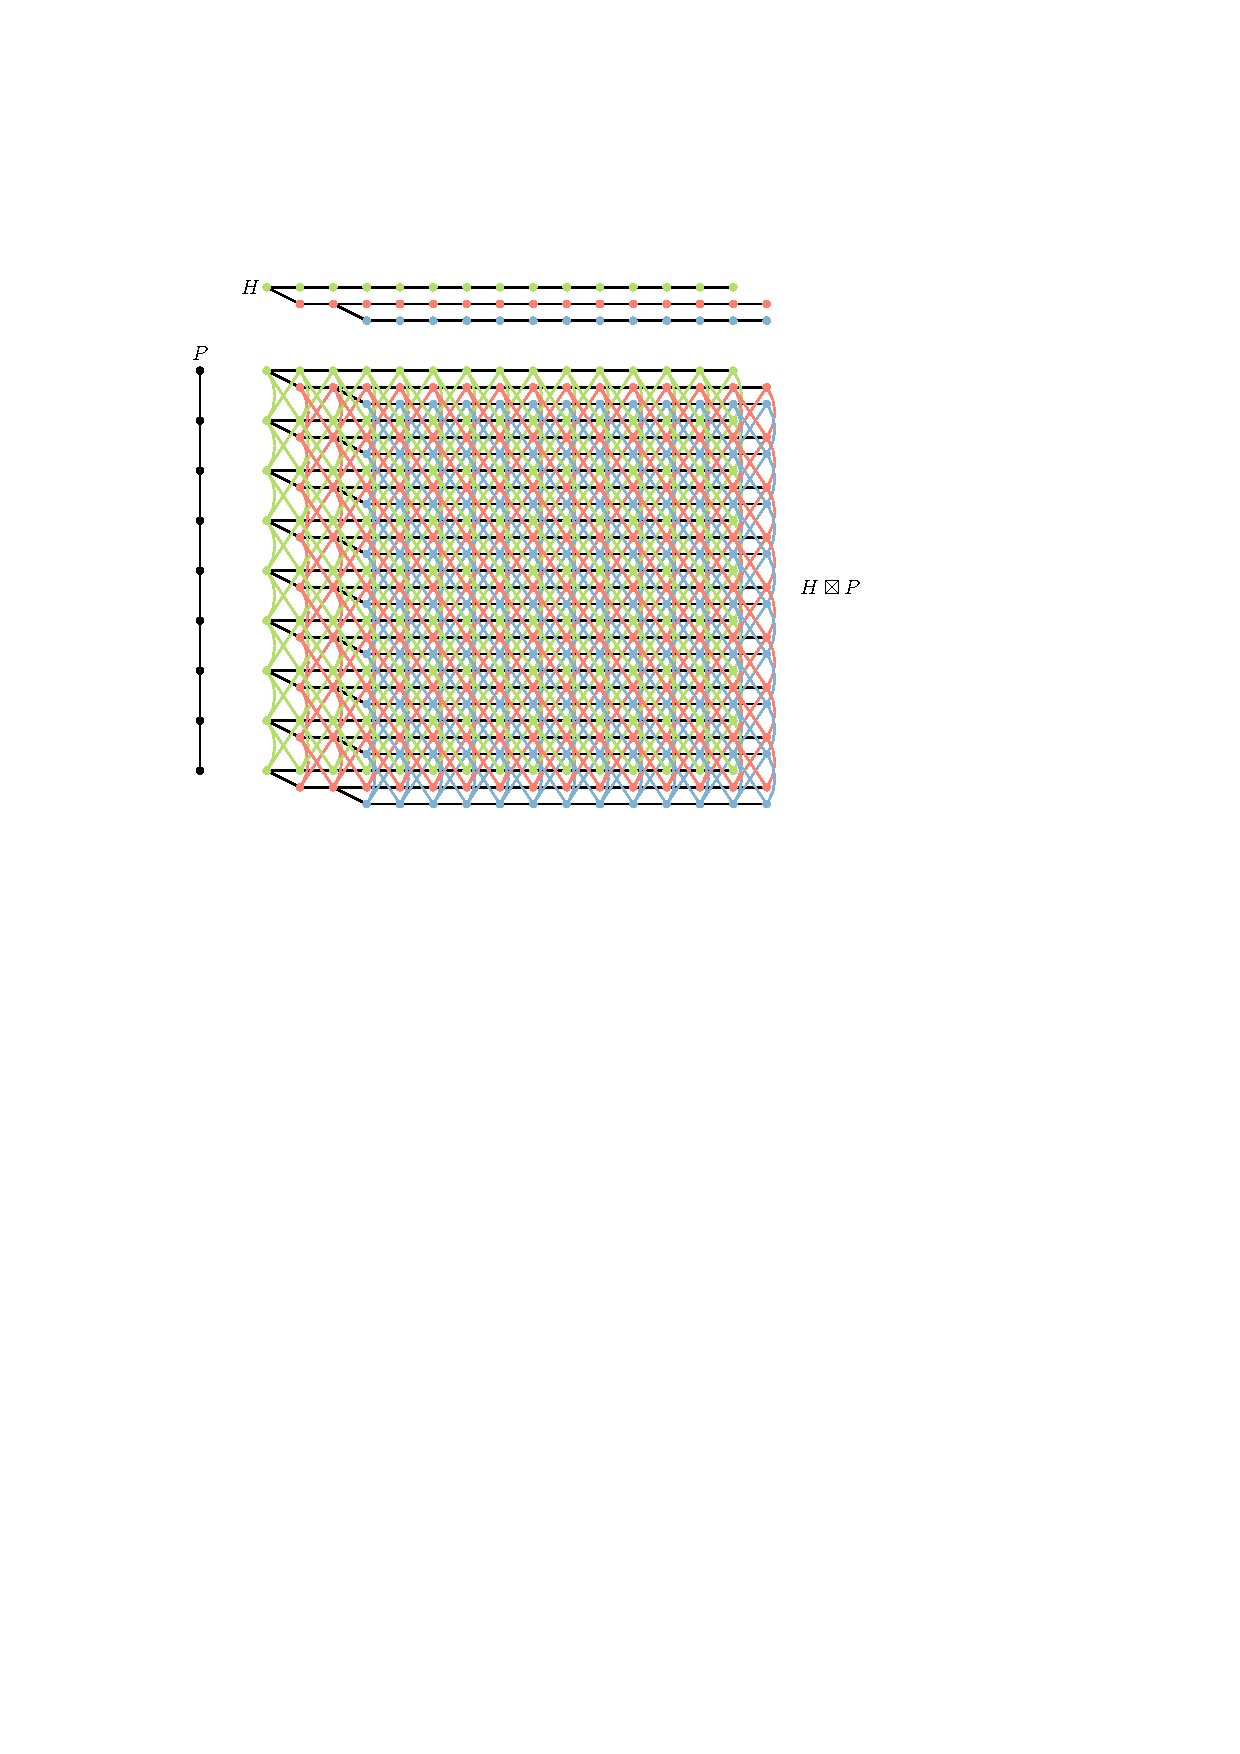
\includegraphics[height=.3\textheight]{figs/product}}%
  \end{center}
  \begin{itemize}[<+->]
    \item Does the same result hold for $G\subseteq H\boxtimes P$?
    \item[$\surd$] Local sparsification: $\ld(G-X)\le D \Leftrightarrow |X|\in O((n\log n)/D)$
    \item[$\surd$] bandwidth of $G-X$ (stuck with Feige):
    $\ld(G)\le D \Rightarrow \bw(G)\in O(D\log^3 n\sqrt{\log n\log\log n})$
    \item For any $G\subseteq H\boxtimes P$,
    \only<4>{$G\subseteq F\boxtimes K_{O(n\log^2 n(\log n\log\log n)^{1/4})}$}%
    \only<5->{$G\subseteq F\boxtimes K_{O(n\log^2 n{\color{red}(\log n\log\log n)^{1/4}})}$}%
    \item (Immediate) applications: bounded-genus graphs, apex-minor-free graphs, $k$-planar graphs, \ldots
    \item Application: proper minor-closed graph classes
  \end{itemize}
\end{frame}

\begin{frame}
  \frametitle{Proper minor-closed graph classes}
  % \framesubtitle{Planar graphs and beyond}

  \textbf{Theorem:} For every proper minor-closed graph class $\mathcal{G}$, every $n$-vertex $G\in\mathcal{G}$ is a subgraph of $F\boxtimes K_{\tilde{O}(\sqrt{n})}$, where $F$ is a \textcolor{red}{fan}.\\[2ex]%

  Proof uses product structure version of GMST.
\end{frame}

\begin{frame}
  \frametitle{Tightening things up}
  % \framesubtitle{Planar graphs and beyond}

  \begin{itemize}
    \item Feige: For \emphh{any} $G$, $\ld(G)\le D$ implies $\bw(G)\in O(D\log^3 n\sqrt{\log n\log\log n})$

    \item Rao (Better): For \emphh{planar} $G$, $\ld(G)\le D$ implies $\bw(G)\in O(D\log^3 n)$

    \item<2-> Here: For  $G\subseteq H\boxtimes P$, $\ld(G)\le D$ implies $\bw(G)\in O(D\log^3 n)$
  \end{itemize}
\end{frame}


\begin{frame}
  \frametitle{Techniques}
  % \framesubtitle{Planar graphs and beyond}

  \begin{center}
  \only<1>{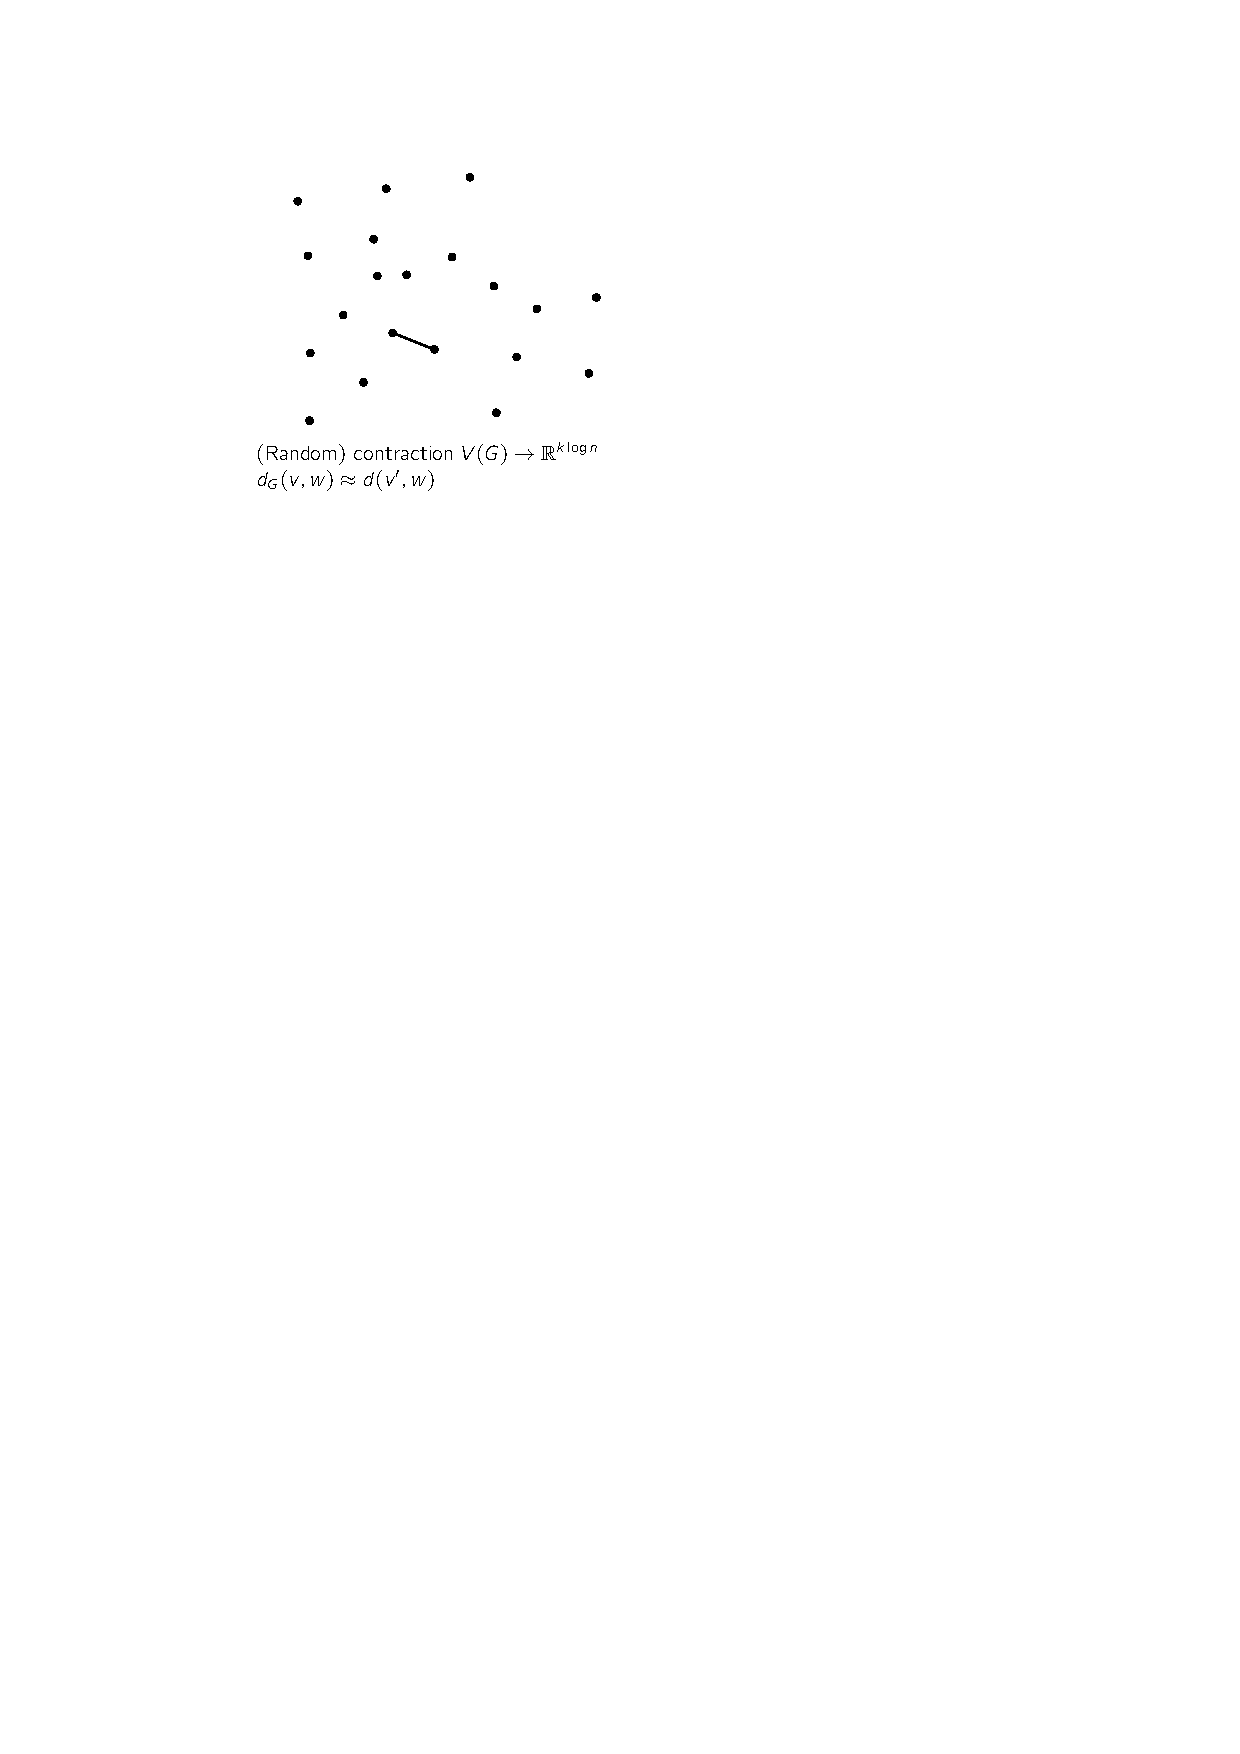
\includegraphics[page=1]{figs/techniques}}%
  \only<2>{\includegraphics[page=2]{figs/techniques}}%
  \only<3>{\includegraphics[page=3]{figs/techniques}}%
  \only<4>{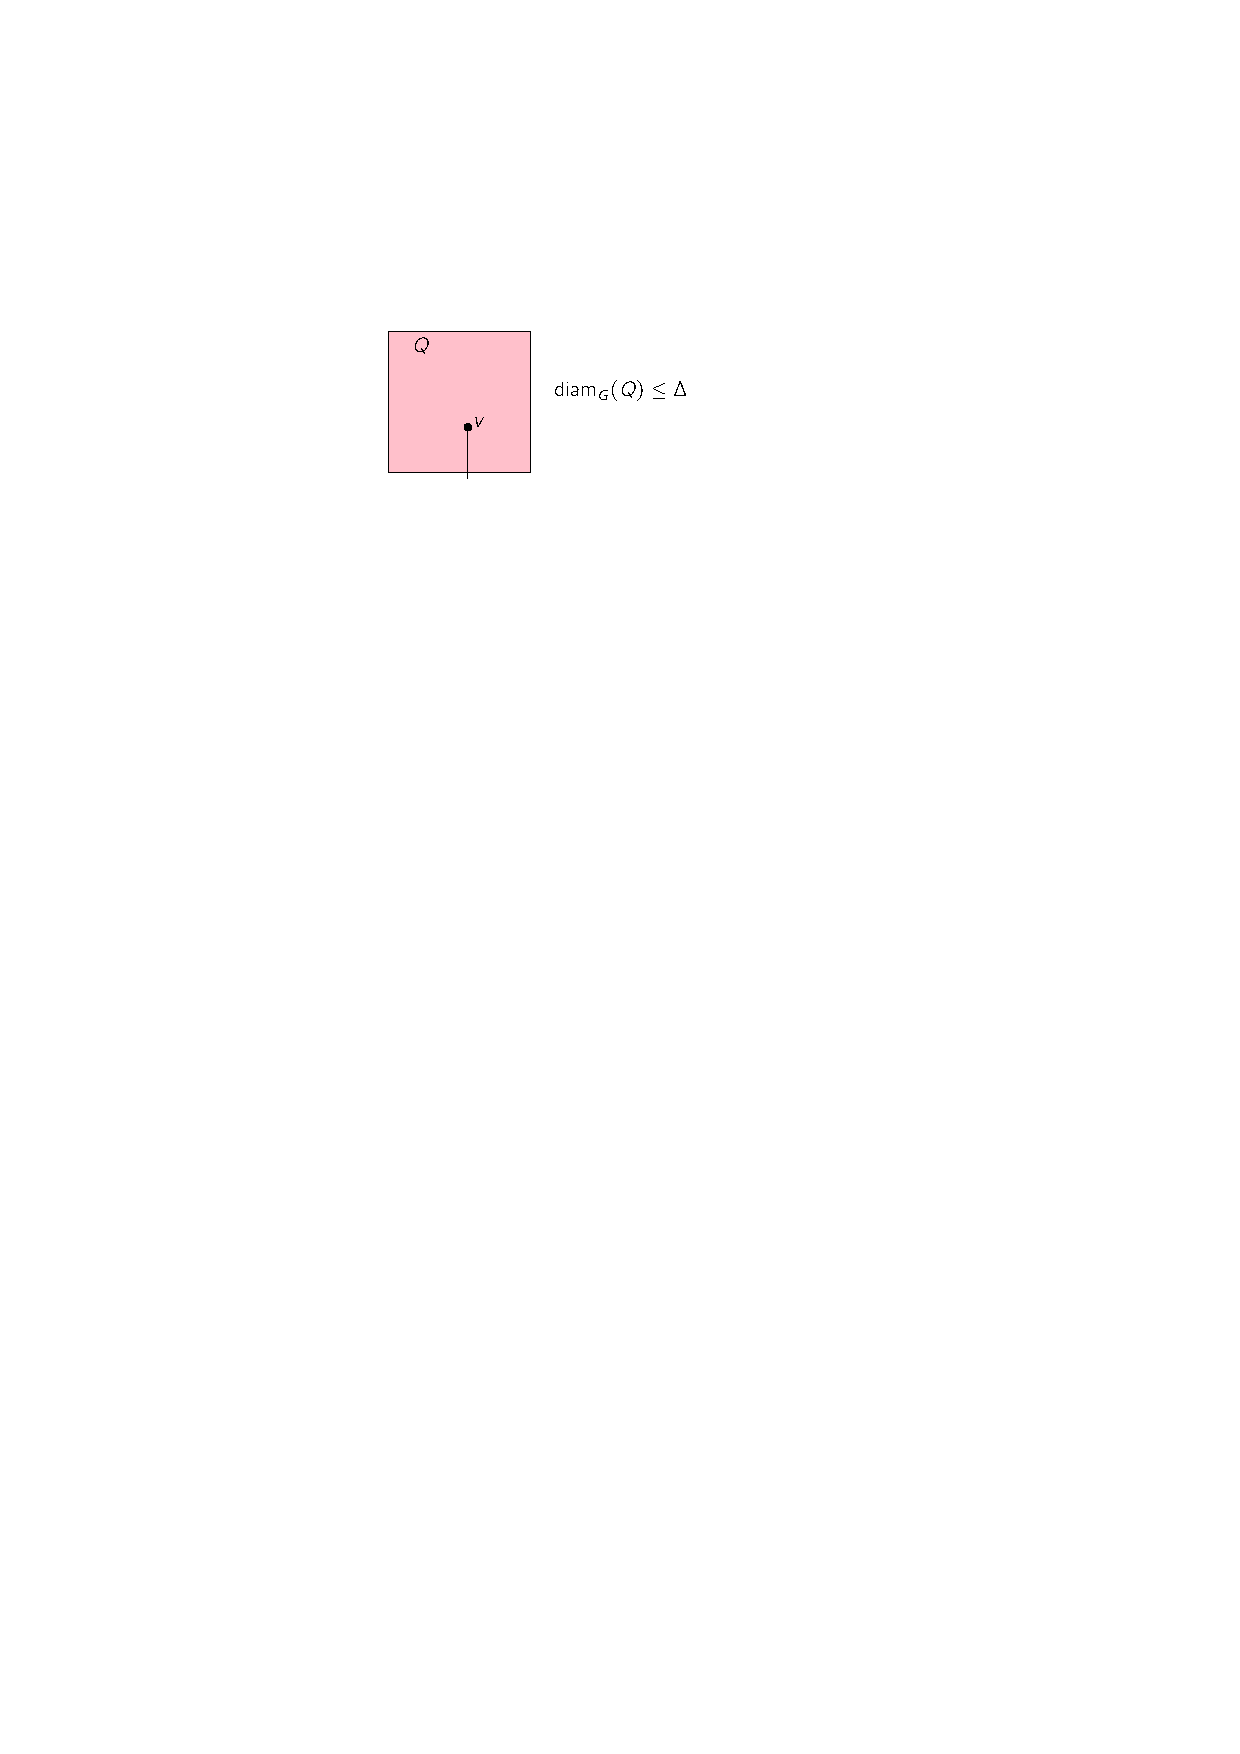
\includegraphics[page=1]{figs/techniques-ii}}%
  \only<5>{\includegraphics[page=2]{figs/techniques-ii}}%
  \only<6>{\includegraphics[page=3]{figs/techniques-ii}}%
  \only<7>{\includegraphics[page=4]{figs/techniques-ii}}%
  \only<8>{\includegraphics[page=5]{figs/techniques-ii}}%
  \only<9>{\includegraphics[page=6]{figs/techniques-ii}}%
  \only<10>{\includegraphics[height=.6\textheight,page=2]{figs/product}}%
  \end{center}
\end{frame}


\begin{frame}
  \frametitle{Complications}
  % \framesubtitle{Planar graphs and beyond}

  \begin{itemize}
    \item We work with distances in $H\boxtimes P$
    \item Each piece $Q$ has $\diam_{H\boxtimes P}(Q)\le \Delta$, not $\diam_{(H\boxtimes P)-X}(Q)\le \Delta$.
    \item Requires new distance function ``between'' $\dist_{H\boxtimes P}$ and $\dist_{(H\boxtimes P)-X}$
    \item Requires generalizing results of Feige from graph metrics to general metrics
  \end{itemize}
\end{frame}


\begin{frame}
  \frametitle{Summary}


  \uncover<1->{Results for product structured and proper-minor closed:\\ $G\subseteq F\boxtimes K_{O(\sqrt{n}\log^2 n)}$} \\[2ex]

  \uncover<2->{Relation to a ``quasi-isometric product structure theorem''}

  \uncover<3->{\textbf{Open Problem:} Get rid of $\log^2 n$ factor?}

  \uncover<4->{\Huge\bf Thank You!}

\end{frame}


\end{document}

\end{document}
